\section{HC1 Architecture \& Overview}

Die HC1 CPU ist ein simpler 8 Bit Rechner. Er ist fähig 10 verschiedene Operationen durchzuführen und stellt einen 32 Byte Speicher zur Verfügung.

\subsection{Block \& RTL Diagram}

\vspace{1em}
\begin{minipage}{\linewidth}
    \centering
    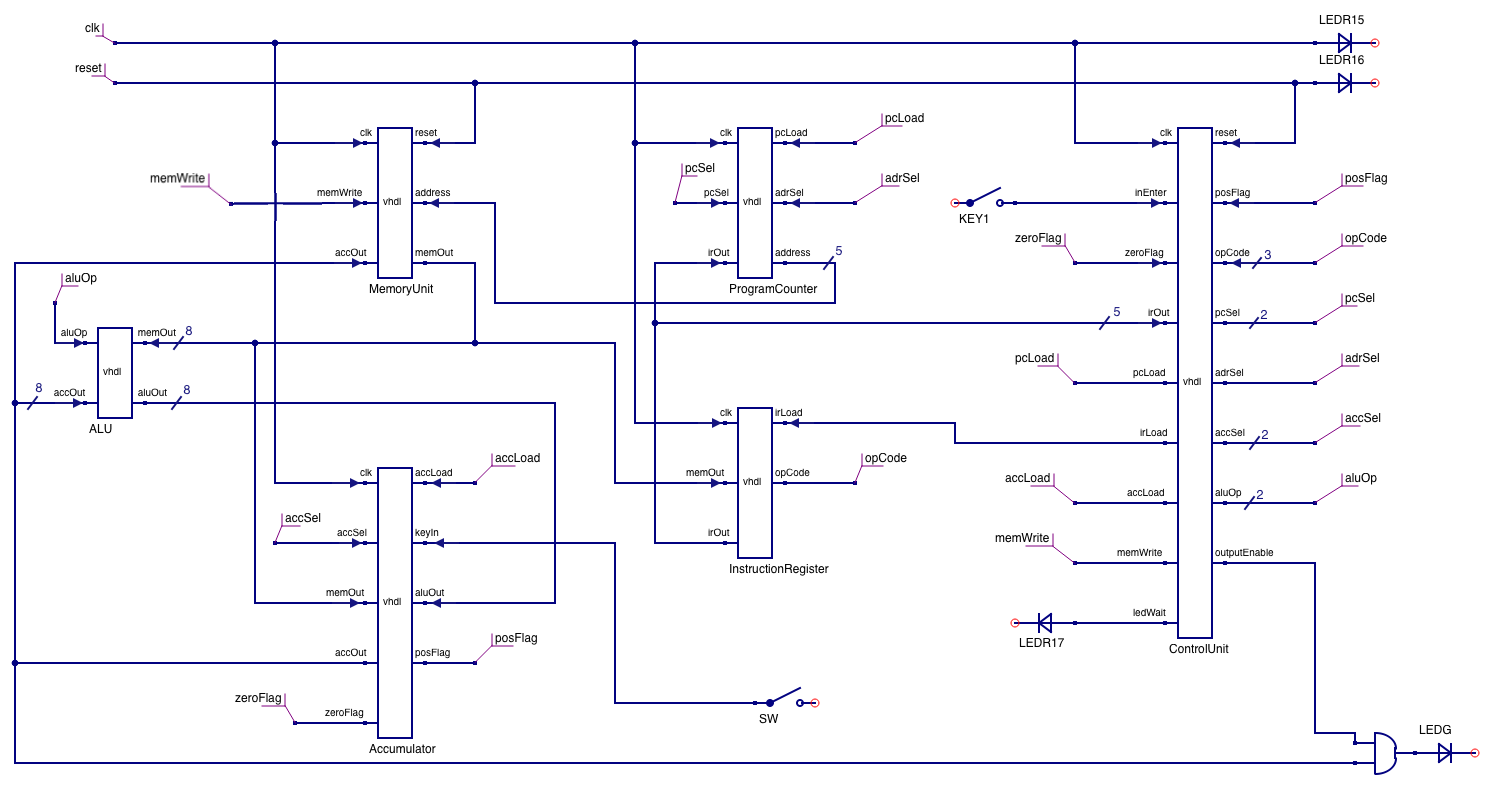
\includegraphics[width=1.0\linewidth]{images/cpu_block.png}
    \captionof{figure}[HC1 Architektur Diagramm]{HC1 Architektur Diagramm}
    \label{fig:block_diagram}
\end{minipage}

Das Diagramm zeigt die Bausteine des HC1 Rechners. Diese werden durch eine CPU Entität über Signale verknüpft.

Die CPU besteht aus den folgenden Bausteinen:

\begin{itemize}
	\item Accumulator
	\item Arithmetic Logical Unit (ALU)
	\item Control Unit
	\item Instruction Register
	\item Memory Unit
	\item Program Counter
\end{itemize}

\vspace{1em}
\begin{minipage}{\linewidth}
    \centering
    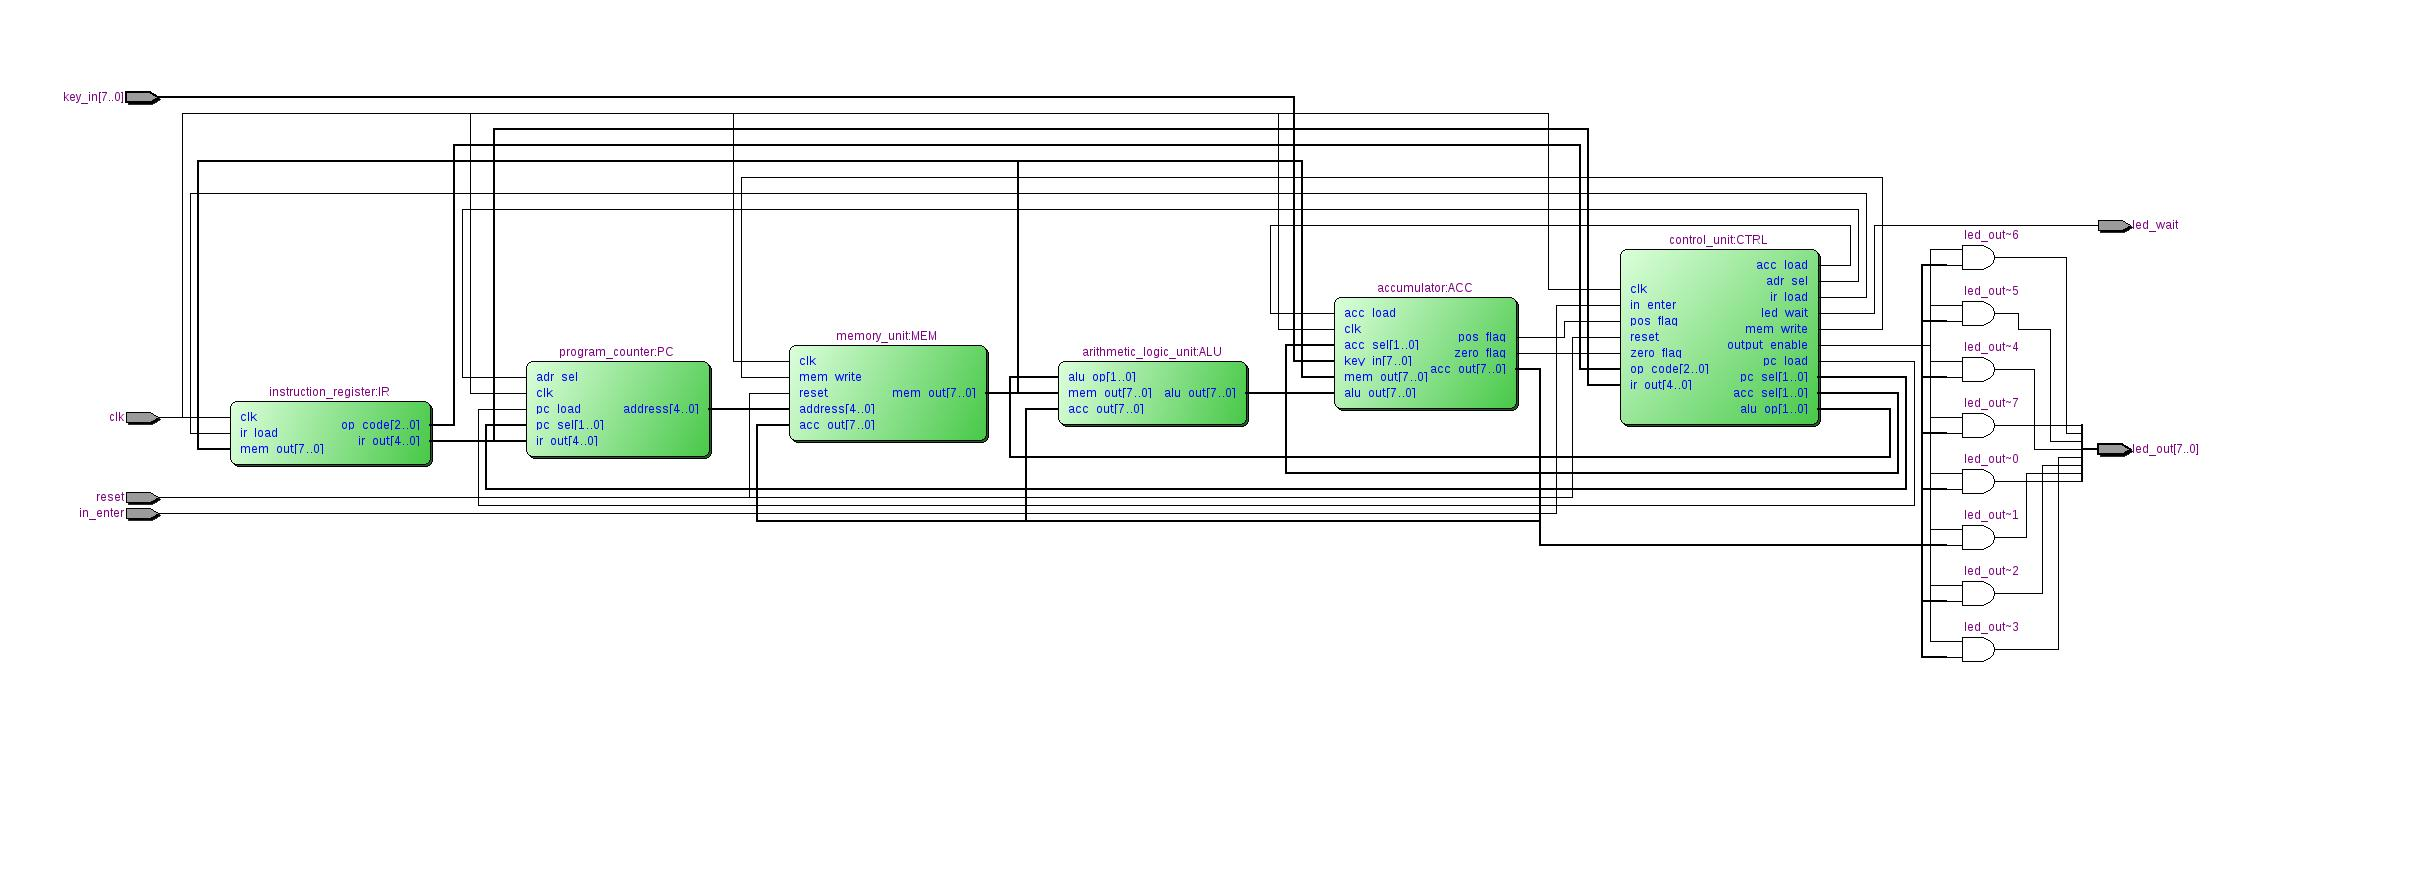
\includegraphics[width=1.0\linewidth]{images/rtl.jpg}
    \captionof{figure}[RTL Diagramm]{RTL Diagramm}
    \label{fig:rtl_diagram}
\end{minipage}


\subsection{Instruction Set}

Der Befehlssatz des Rechner besteht aus 10 verschiedenen Instruktionen.

Jeder Befehl enthält hierbei 3 Op-Code Bits und 5 Adress Bits.

\vspace{1em}
\begin{table}[!h]
	\centering
	\begin{tabular}{|l|c|c|c|}
		\hline
		\textbf{Befehl} & \textbf{OpCode} & \textbf{Data} & \textbf{Taktzyklen}\\
		\hline
		\texttt{LOAD} & \texttt{000} & \texttt{aaaaa} & 5 \\
		\hline
		\texttt{STORE} & \texttt{001} & \texttt{aaaaa} & 5 \\
		\hline
		\texttt{ADD} & \texttt{010} & \texttt{aaaaa} & 5 \\
		\hline
		\texttt{SUB} & \texttt{011} & \texttt{aaaaa} & 5 \\
		\hline
		\texttt{NAND} & \texttt{100} & \texttt{eeeee} & 5 \\
		\hline
		\texttt{IN} & \texttt{100} & \texttt{00000} & 5 \\
		\hline
		\texttt{OUT} & \texttt{100} & \texttt{00001} & 5 \\
		\hline
		\texttt{JZ} & \texttt{101} & \texttt{aaaaa} & 4 \\
		\hline
		\texttt{JPOS} & \texttt{110} & \texttt{aaaaa} & 4 \\
		\hline
		\texttt{J} & \texttt{111} & \texttt{aaaaa} & 4 \\
		\hline
	\end{tabular}
	\caption{Instruction Set}
	\label{tab:instruction_set}
\end{table}

\textbf{Taktzyklen:}

Die dargestellte Takzyklenanzahl der Befehle kann zwischen verschiedenen Implementationen abweichen.

\textbf{Daten:}

Die angegebene Datenkodierung stellt folgende Werte dar:

\begin{enumerate}
\item \texttt{aaaaa} - Adresse im Bereich 0 - 32
\item \texttt{eeeee} - Adresse im Bereich 2 - 32
\end{enumerate}

\subsubsection{Befehle}

Folgend eine kurze Finktionsbeschreibung der Befehle:

\paragraph{LOAD} Lädt einen Wert aus dem Hauptspeicher in den Akkumulator.

\paragraph{STORE} Speichert einen Wert aus dem Akkumulator in den Hauptspeicher.

\paragraph{ADD} Addiert einen Wert aus dem Hauptspeicher zu dem Wert im Akkumulator.

\paragraph{SUB} Subtrahiert einen Wert aus dem Hauptspeicher von dem Wert im Akkumulator.

\paragraph{NAND} Führt eine NAND Operation mit dem Wert im Hauptspeicher und dem Akkumulatorwert durch.

\paragraph{IN} Speichert eine Eingabe im Akkumulator.

\paragraph{OUT} Setzt den aktuellen Akkumulatorwert auf den Ausgangsbus.

\paragraph{JZ} Führt eine Sprunganweisung durch, wenn der Akkumulatorinhalt gleich 0 ist (zeroFlag).

\paragraph{JPOS} Führt eine Sprunganweisung durch, wenn der Akkumulatorinhalt größer 0 ist (posFlag).

\paragraph{J} Führt eine Sprunganweisung durch..

\subsection{Default Program \& Simulation}

\vspace{1em}
\begin{minipage}{\linewidth}
    \centering
    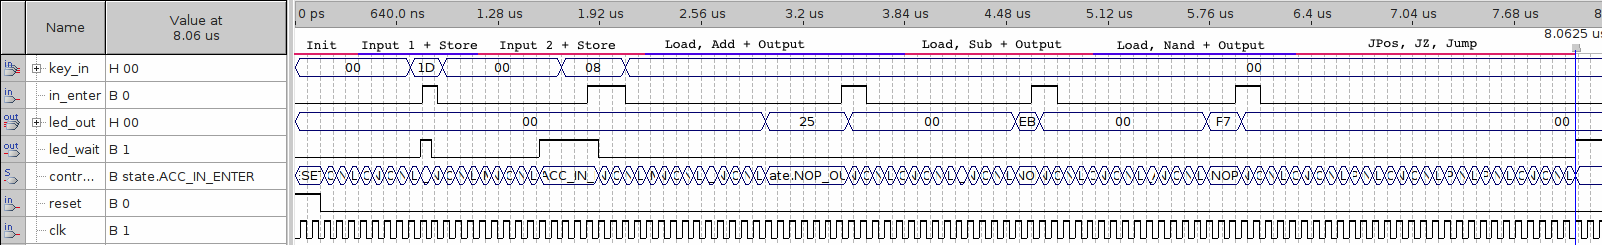
\includegraphics[width=1.0\linewidth]{images/sim.png}
    \captionof{figure}[Program Simulation]{Program Simulation}
    \label{fig:simulation}
\end{minipage}

\subsection{Modifikationen}
\label{modifications}

Hier werden die Abweichungen zur originalen HC1 Vorlage beschrieben.

\paragraph{ledWait}

Das im Blockdiagram \ref{fig:block_diagram} zu sehende Signal \emph{ledWait} wurde von mir hinzugefügt und ist nicht Bestandteil des ursprünglichen HC1 Rechners. Es dient zur Darstellung einer Eingabeaufforderung.